\section*{Discussion}

% Accumulation of RecA filaments at high cipro might be due to extensive DNA damage and unsuccessful homology search
\subsection*{Accumulation of RecA filaments under high DNA damage}
Under exposure to high ciprofloxacin concentrations (20-30 ng/ml), we observed an accumulation of RecA filaments in cells (Figures \ref{Fig:reca_nucleoid}A and \ref{Fig:reca_nucleoid}B). At these ciprofloxacin concentrations, we have determined that cells undergo frequent DSBs, leading to multiple recruitments of RecB to DNA over the course of the experiment (up to 5 per hour, Figure \ref{Fig:recruitment}B). In these conditions, it would become increasingly likely for all copies of a locus to be damaged, and the DSB repair pathway to be stuck at the step of homology searching.

\subsection*{Multiple RecB recruitments per DSB in the $\mathbf{\Delta}$\emph{reca} and RecB$\mathbf{_{1080}}$ mutants}

% Model of RecB recruitment to DNA
\begin{figure*}[htbp]
    \centering
    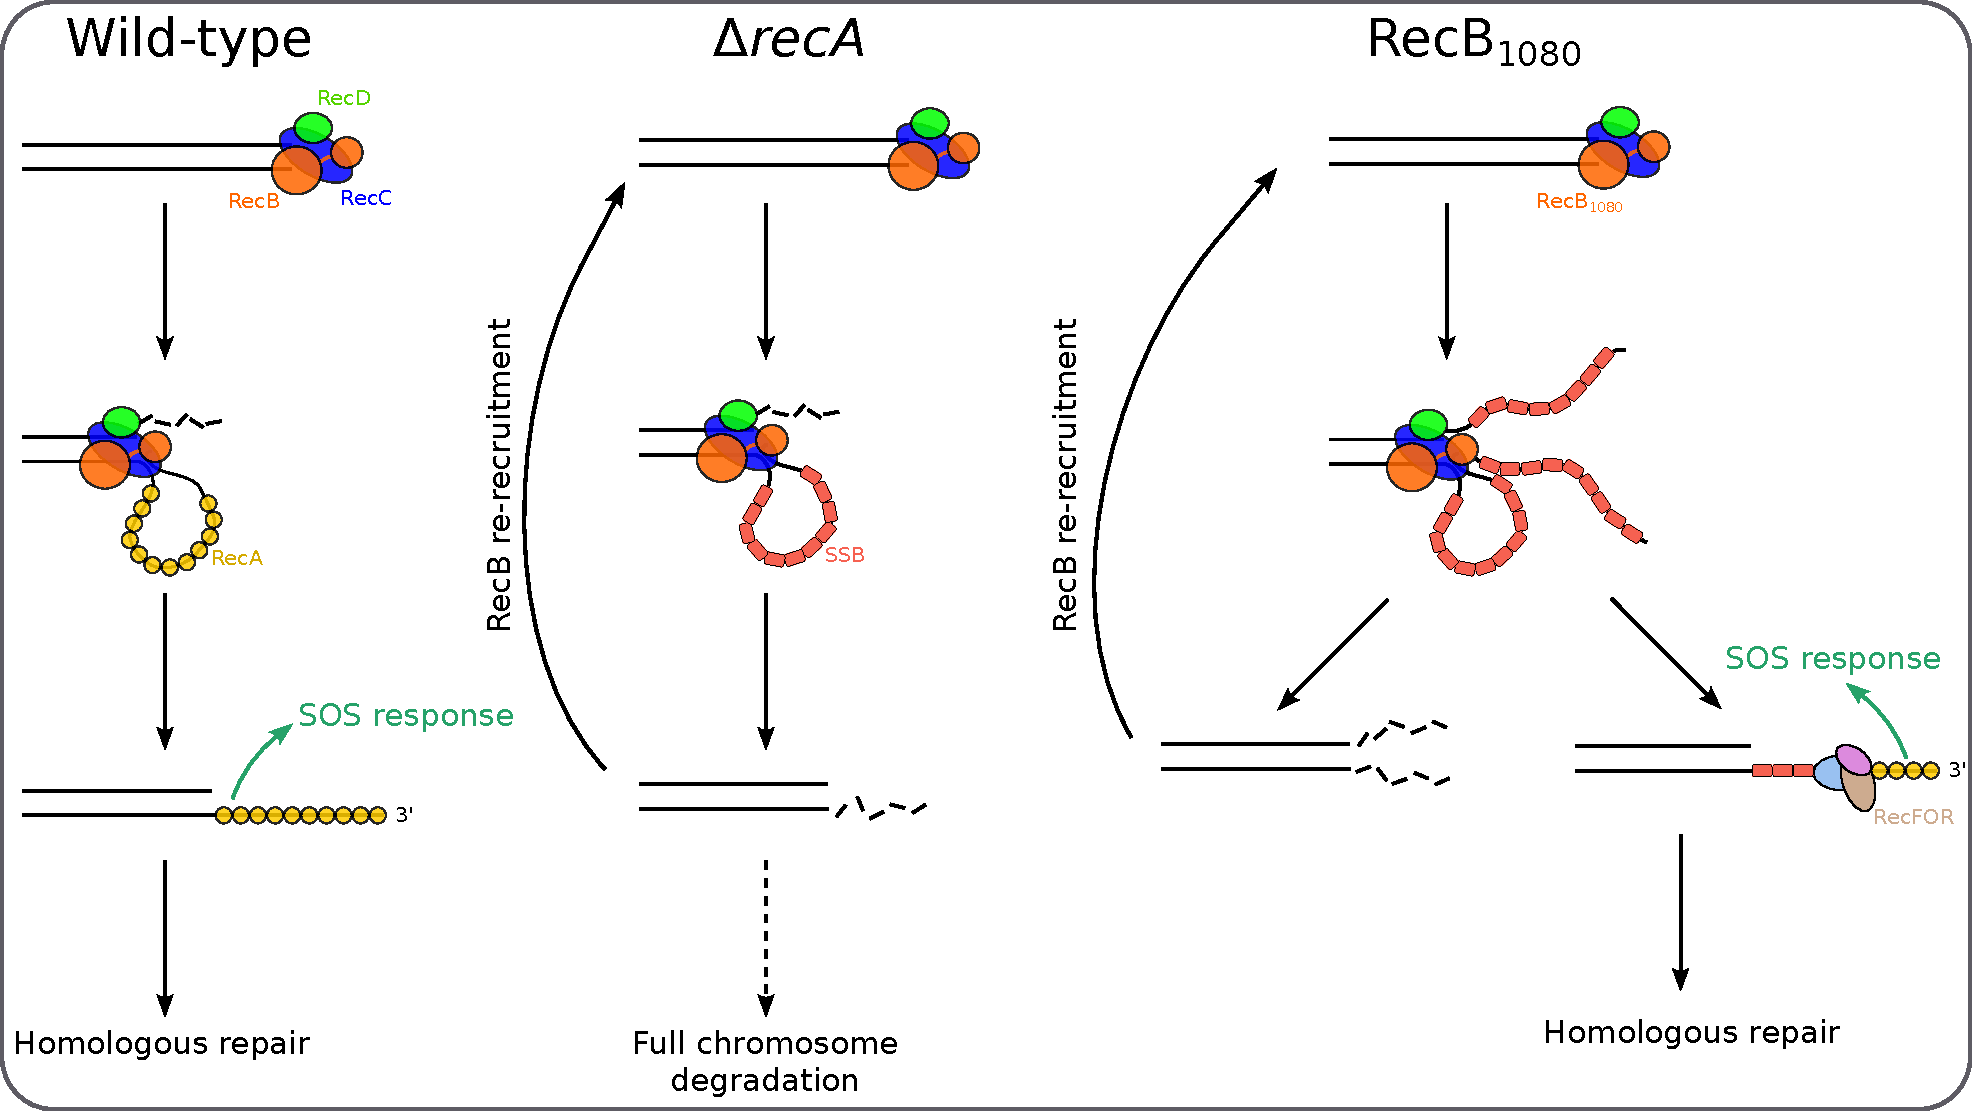
\includegraphics[width=\textwidth]{Figures/Fig_mutants_pathways.pdf}
    \caption{RecBCD recruitment pathways in wild-type \emph{E. coli}, \dreca\ and \geneteneighty\ mutants. \textbf{(Wild-type)} After DSB recognition, RecBCD degrades DNA until it recognises a Chi-site. It switches activity to create a 3' ssDNA overhang, and promotes RecA loading. The RecA-coated ssDNA can then be used for DNA repair by homologous recombination. \textbf{($\mathbf{\Delta}$reca)} In the absence of RecA, the 3' ssDNA is coated by SSB, and eventually digested by cellular nucleases. Blunting of the DNA end by digestion of the ssDNA creates a new substrate for binding of RecBCD. \textbf{(RecB$\mathbf{_{1080}}$)} Following DSB recognition, \teneighty\ unwinds DNA without digesting it. The unwound ssDNA can either be digested by nucleases, leading to a new blunt dsDNA end and RecBCD re-recruitment; or the RecFOR complex displaces SSB to load RecA, allowing DNA repair by homologous recombination to proceed.}
    \label{Fig:pathways}
\end{figure*}

Our observations of cell elongation (Figure \ref{Fig:mutants}A), RecB recruitment to DNA (Figure \ref{Fig:mutants}C), and nucleoid position (Figure \ref{Fig:mutants}D) in the different mutant strains have led us to the model of RecB recruitment described in Figure \ref{Fig:pathways}. In wild-type cells, a DSB is recognised by RecBCD, which promotes RecA loading. The RecA filament triggers the SOS response, and is used for homology search and repair. In the \dreca\ mutant, the 3' ssDNA generated by RecBCD is first coated by SSB, and then degraded by cellular nucleases. This leads to blunting of the DNA end, creating a new substrate on which RecBCD can bind. This circle leads to multiple RecBCD recruitments per DSB, and eventually to full chromosome degradation. In the \geneteneighty\ mutant, RecBCD unwinds DNA without degrading it. After the ssDNA is coated with SSB, two competing pathways take place: either DNA degradation by nucleases leading to DNA-end blunting and re-recruitment of RecBCD, or displacement of SSB by RecFOR and loading of RecA, leading to SOS induction and homologous repair.

% Linking the RecB recruitment rate to DSB formation rate (ok in WT, more difficult in mutants due to re-recruitment to the same DSB)
\subsection*{Extrapolating the rate of DSB formation from the number of recruitments of RecB to DSBs}
Our experiments allowed us to estimate the number of recruitment of RecB to DSBs per hour, under different ciprofloxacin concentrations (Figure \ref{Fig:recruitment}B), and in the \dreca\ and \geneteneighty\ mutants (Figure \ref{Fig:mutants}C). In the wild-type, the general pathway for DSB repair suggests that RecBCD is recruited once per DSB (Figure \ref{Fig:pathways}). We can therefore reasonably expect that the observed number of RecB recruitments observed matches with the number of DSBs formed (between 1 to 5 per hour, depending on ciprofloxacin concentration). In the \dreca\ and \geneteneighty\ mutants however, the disruptions to the DSB repair pathway lead to multiple RecB recruitments per DSB. We are therefore not able to estimate the rate of DSB formation in these mutants.

It should be noted that ciprofloxacin is expected to produce double-sided DSBs, hence leading to two RecB recruitments per break. We did not take this into account in our estimation of the DSB formation rate, as it has been previously suggested that the two sides of a DSB are kept in close proximity during DNA repair\cite{Vickridge2017,Keyamura2019}, and our imaging setup would not allow us to separate two RecB spots located close together. Indeed, our timelapse images of RecB binding seldom show two spots next to each other, further supporting the idea that we are not able to resolve RecBCD binding to both sides of a DSB.
